\documentclass[a4paper,11pt]{article}
% ---- graphiques
\usepackage[pdftex]{graphicx}
\usepackage{wrapfig}
\usepackage{color}
%\usepackage{hyperref}

% for latex2html
\usepackage{html}

% for accents
\usepackage[latin1]{inputenc}
\usepackage[T1]{fontenc}

\usepackage{algorithm}
\usepackage{algorithmic}

\definecolor{darkgreen}{rgb}{0,0.4,0}
\definecolor{darkblue}{rgb}{0,0,0.4}
\definecolor{darkgray}{rgb}{0.2,0.2,0.2}

% ---- inclusion de codes
\usepackage{listings}
\lstset{showstringspaces=false,tabsize=4,basicstyle=\scriptsize\sffamily,breaklines=true,breakatwhitespace=true,framexleftmargin=5mm, frame=shadowbox, framesep=1pt,rulesepcolor=\color{darkgray},rulesep=.5pt,keywordstyle=\bf\color{blue},commentstyle=\color{magenta},stringstyle=\color{red},numbers=left,numberstyle=\tiny,numbersep=5pt,columns=flexible}

\lstdefinestyle{bash}{language=bash}
\lstdefinestyle{Perl}{language=Perl}
\lstdefinestyle{C++}{language=C++,emph={__global__,__shared__,__syncthreads,blockIdx,threadIdx,float3,float4},emphstyle=\bf\color{darkgreen}}
\lstdefinestyle{DTD}{language=XML}
\lstdefinestyle{XML}{language=XML,usekeywordsintag=false,markfirstintag=true}
%begin{latexonly}
\newcommand{\includecode}[2]{
\lstinputlisting[style=#1]{#2}
}
%end{latexonly}
\begin{htmlonly}
\newcommand{\includecode}[2]{  \htmladdnormallink{#2}{../../#2} }
\end{htmlonly}

%\lstnewenvironment{code}{}{}
\lstnewenvironment{code_bash}{\lstset{style=bash}}{}
\lstnewenvironment{code_perl}{\lstset{style=Perl}}{}
\lstnewenvironment{code_cpp}{\lstset{style=C++}}{}
\lstnewenvironment{code_dtd}{\lstset{style=DTD}}{}
\lstnewenvironment{code_xml}{\lstset{style=XML}}{}

\newcommand{\textcode}[1]{{\sf #1}}



%
\newcommand{\sofa}{SOFA}
\newcommand{\todo}[1]{}
\newcommand{\eg}{\textit{e.g.} }

\renewcommand{\vec}[1]{\ensuremath{\mathbf{#1 }}} % vector
\newcommand{\Vx}{\vec{x} } % position vector
\newcommand{\Vv}{\vec{v} } % velocity vector
\newcommand{\Va}{\vec{a} } % acceleration vector
\newcommand{\Vf}{\vec{f}} % force
\newcommand{\Vdv}{\vec{\delta\Vv}} % change of velocity vector (unknown in implicit CG, and used in constraint solver
\renewcommand{\P}{\mat{P} } % projection to a constrained space.

\newcommand{\JNL}{\mathbf{\mathcal{J}} }     % mapping des positions
\newcommand{\J}{\mat J }                 % mapping lineaire
\newcommand{\M}{\mat M }             % matrice de masse
\newcommand{\K}{\mat K }             % matrice de raideur
\newcommand{\B}{\mat B }             % matrice d'amortissement
\newcommand{\G}{\mat G }             % jacobien des contraintes



% ---- inclusion de codes
\definecolor{darkgreen}{rgb}{0,0.4,0}
\definecolor{darkblue}{rgb}{0,0,0.4}
\definecolor{darkgray}{rgb}{0.2,0.2,0.2}


% macros mathematiques
\newcommand{\ma}[1]{\ensuremath{\mathbf {#1}}}
\newcommand{\ve}[1]{\ensuremath{\mathbf {#1}}}

\usepackage{amsmath}
\usepackage{amsfonts}
\usepackage{amssymb}

% character styles
\newcommand{\bm}[1]{\ensuremath{\mathbf{{#1}}}}
\newcommand{\mcal}[1]{\mbox{$\mathcal #1$}} % rondes math
\newcommand{\bmcal}[1]{\mbox{\boldmath $\mathcal #1$}} % rondes grasses math
\newcommand{\ensemble}[1]{\mbox{$\mathbb{#1}$}}
\newcommand{\RRR}{\mbox{$\ensemble{R}^3$}} 


 % This file is in parent directory. Your TEXINPUTS environment variable must include .. to reach this file. Example: setenv TEXINPUTS ..:../..:${TEXINPUTS}

% ---- format de page A4
	\setlength{\textwidth }{16cm}	% largeur de ligne
	\setlength{\textheight}{23cm}   % hauteur du texte
	\setlength{\oddsidemargin}{0cm} % marge pages impaires
	\setlength{\evensidemargin}{0cm}% marge pages paires
	\setlength{\topmargin}{0cm} 	
	\setlength{\headheight}{14pt} 
	\setlength{\headsep}{0.5cm} 


% Title Page
\title{\sofa}
\author{The \sofa{} team}
\date{2007}
% \author{Fran\c{c}ois Faure\\ J\'er\'emie Allard\\ {\small INRIA Rh\^one-Alpes, Grenoble, France}}

\begin{document} 
\maketitle

\begin{abstract}
In this document we explain the usage and the fucntionalities of the modules developped using the Core Sofa Framework.

\end{abstract}

\section{Collision Models}
\subsection{Ray Traced Collision Detection}
This module implements the algorithm described in the paper entitled "Ray-traced collision detection for deformable bodies" by E.Hermann F.Faure and B.Raffin. When two objects are in collision, a ray is shot from each surface vertex in the direction of the inward normal. A collision is detected when the first intersection belongs to an inward surface triangle of another body.  A contact force between the vertex and the matching point is then created. Experiments  show that this approach is fast and more robust than traditional proximity-based collisions.

 To speedup the  searching of elements that cross the ray,   we  stored all the triangles of each colliding objects in an  octree. Therefore we can easily navigate inside this octree and efficiently find the points crossing the ray. The octree structure allow us to have a satisfying performance independently from the size of the triangles used, which is not the case for  a regular grid.


\subsubsection{Using this module}
An example showing the usage of the Ray Traced collision detection can be found in the  RayTraceCollision.scn file in the \textit{scene} directory. The collision detection mechanism must be set as \textbf{RayTraceDetection}, and instead of using a TriangleModel one must use a \textbf{TriangleOctreeModel}. The TriangleOctreeModel will create an Octree that contains all the Triangles from the collision model. 
	

\section{Forces}
\subsection{NonUniformHexahedronFEMForceFieldAndMass}
\graphicspath{{../modules/}}  % to include images


\subsubsection{Concepts}

This force field implement the article :

\begin{verbatim}
      @InProceedings{NPF06,
      author       = "Nesme, Matthieu and Payan, Yohan and Faure, Fran\c{c}ois",
      title        = "Animating Shapes at Arbitrary Resolution with Non-Uniform Stiffness",
      booktitle    = "Eurographics Workshop in Virtual Reality Interaction and Physical Simulation (VRIPHYS)",
      month        = "nov",
      year         = "2006",
      organization = "Eurographics",
      address      = "Madrid",
      url          = "http://www-evasion.imag.fr/Publications/2006/NPF06"}
 \end{verbatim}
 
 
 
The basic idea, illustrated in figure \ref{fig:condensation}, is :


\begin{figure}
\begin{center}
	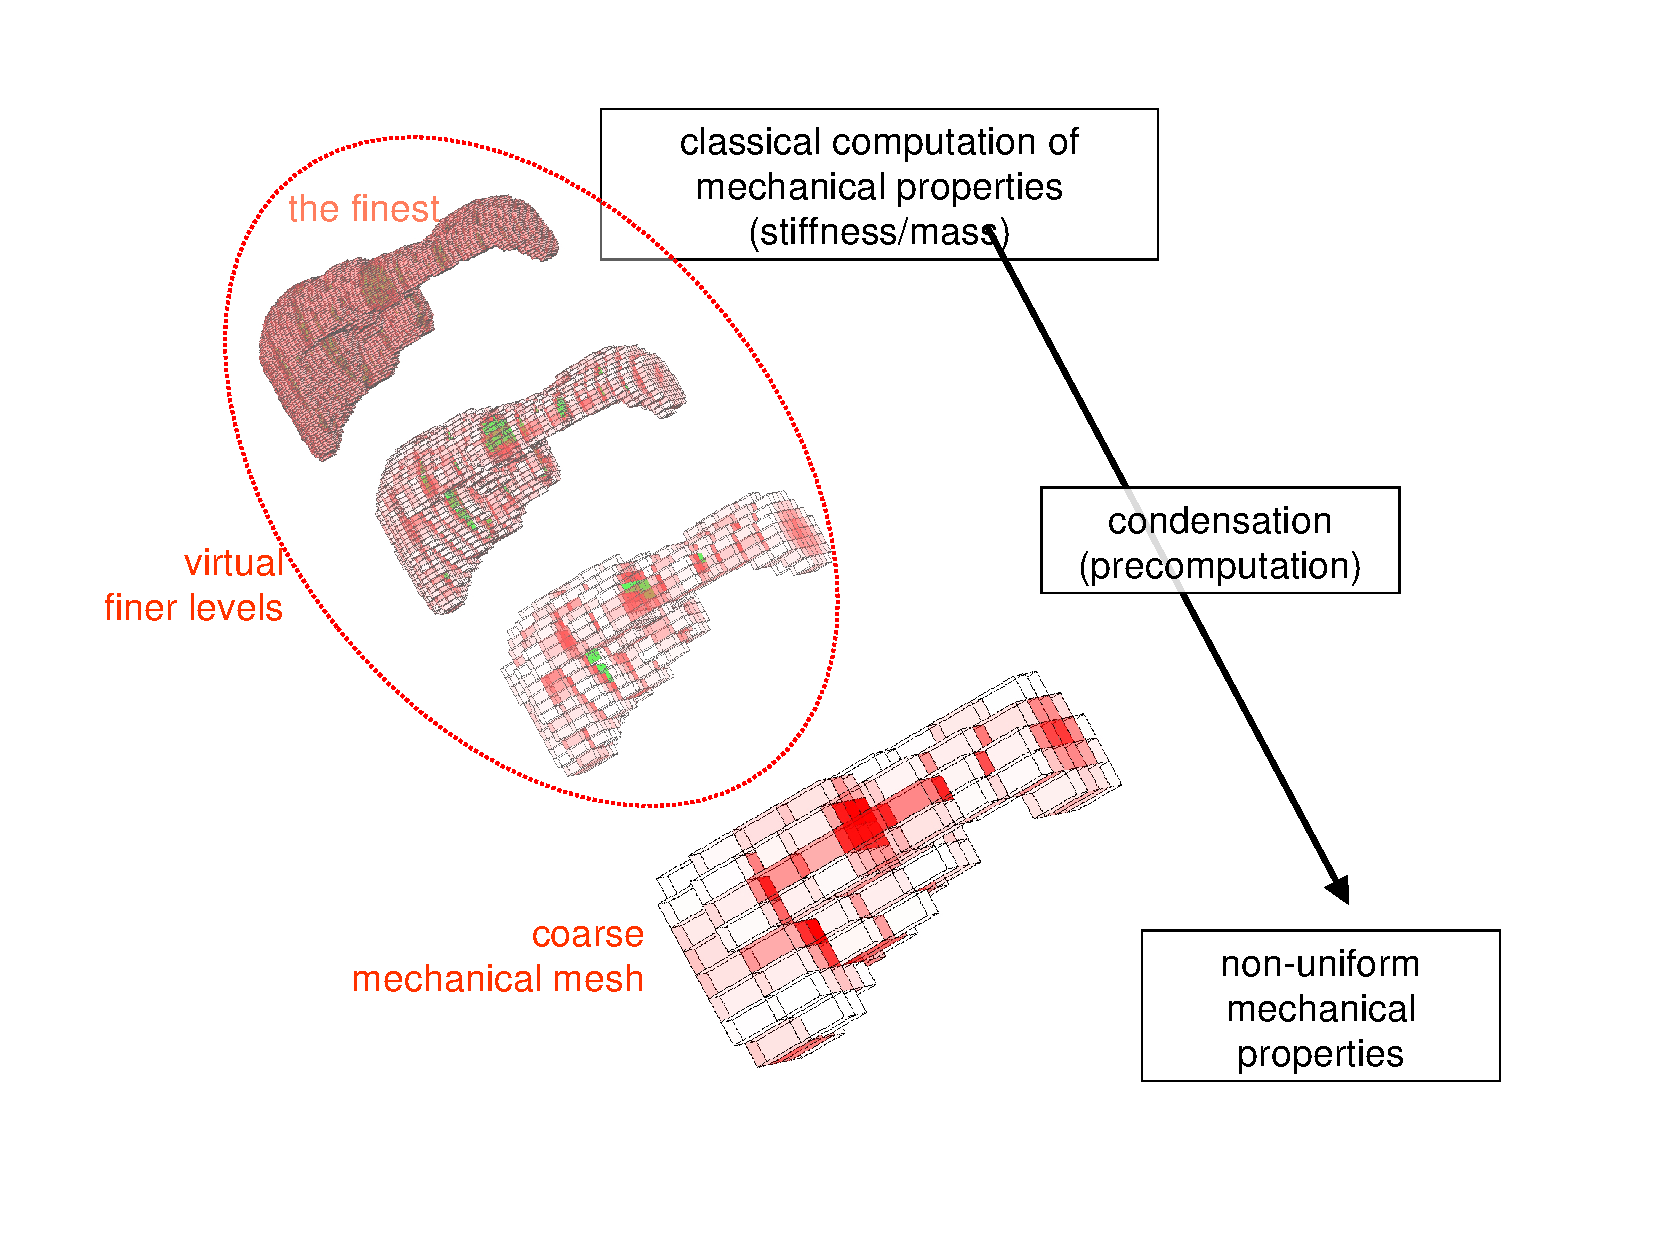
\includegraphics[width=\linewidth]{forcefield/nonUniformHexahedron/condensation.pdf}
\end{center}
	\caption{The condensation principle.}
	\label{fig:condensation}
\end{figure}



\begin{itemize}
\item the use of finer virtual levels of SparseGrid
\item the computation of classical mechanical matrices (mass and stiffness) at the finest resolution and the condensation of theses matrices to the current coarse mechanical resolution
\end{itemize}


\textbf{Warning} : actually the NonUniformHexahedronFEMForceFieldAndMass is only working with SparseGridTopology, and need enough finer virtual levels to compute the condensation. 

\subsubsection{Data Fields}

\begin{itemize}
\item From HexahedronFEMForceFieldAndMass
	\begin{itemize}
	\item method (char) : large/polar, the corotationnal method (default = large)
	\item poissonRatio, youngModulus, density (float) : mechanical properties (density = volumetric mass in english $kg.m^{-3}$)
	\item assembling (bool) : assembling the global system matrix ? (default = false)
	\end{itemize}
\item Specific to NonUniformHexahedronFEMForceFieldAndMass
	\begin{itemize}
	\item nbVirtualFinerLevels (int) : how many finer virtual levels are employed in the condensation stage ? (default = 0)
	\end{itemize}
\item A hack on masses (for debugging)
		\begin{itemize}
	\item useMass (bool) : are the condensated mass matrices are used ? (if not, scalar masses concentrated on particles are used) (default = 0)
	\item totalMass (float) : if useMass=false, the scalar mass of the object
	\end{itemize}
\end{itemize}


\subsubsection{Example}



\begin{verbatim}

<Node name="non uniform">
   <Object type="SparseGrid"
                   n="4 4 4"
                   filename="mesh/mymesh.obj"
                   nbVirtualFinerLevels="2"  />
   <Object type="MechanicalObject"/>
   <Object type="NonUniformHexahedronFEMForceFieldAndMass"
                   nbVirtualFinerLevels="2"
                   youngModulus="20000"
                   poissonRatio="0.3"
                   density="10" />
</Node>

\end{verbatim}

\textbf{Important} : note that the SparseGrid has nbVirtualFinerLevels=2 in order to built enough finer virtual levels. This SparseGrid$->$nbVirtualFinerLevels has to be greater or equal to the NonUniformHexahedronFEMForceFieldAndMass$->$nbVirtualFinerLevels.
\\

A more complex example can be found in : examples/Components/forcefield/NonUniformHexahedronFEMForceFieldAndMass.scn where a comparison with a classical HexahedronFEMForceFieldAndMassForceField is done.



\section{Soft Articulations}


\subsection{Concepts}

The objective of this method is to use stiff forces to simulate joint articulations, instead of classical constraints.
\paragraph{}
To do this, a joint is modeled by a 6 degrees of freedom spring. By the way, the user specify a stiffness on each translation and rotation.
\begin{itemize}
	\item A null stiffness defines a free movement.
	\item A huge stiffness defines a forbidden movement.
	\item All nuances are possible to define semi constrained movements.
\end{itemize}

\paragraph{}
2 main advantages can be extracted from this method :
\begin{itemize}
	\item A better stability. As we don't try to statisfy constraints but only apply forces, there is always a solution to resolve the system.
	\item more possibilities to model articulations are allowed. As the stiffnesses define the degrees of freedom of the articulations, a better accuracy is posssible to simulate free movements as forbidden movements, i.e. an articulation axis is not inevitably totally free or totally fixed.
\end{itemize}



\subsection{Realization}

To define physically an articulated body, we first have a set of rigids (the bones). \textsl{cf fig. 1}
\begin{figure}[hp]
	\centering
		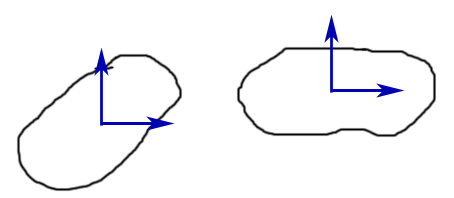
\includegraphics[width=0.30\textwidth]{softArt_G1.png}
	\caption{two bones}
	\label{2 Bones}
\end{figure}


Each of these bones contains several articulations points, also defined by rigids to have orientation information. \textsl{cf fig. 2}
\begin{figure}[htpb]
	\centering
		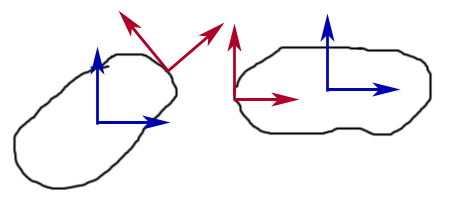
\includegraphics[width=0.30\textwidth]{softArt_G2.png}
	\caption{two bones (blue) with their articulation frames (red)}
\end{figure}

As seen previously, a joint between 2 bones is modeled by a 6-DOF spring. These springs are attached on the articulations points.    \textsl{cf fig. 3}
\begin{figure}[htpb]
	\centering
		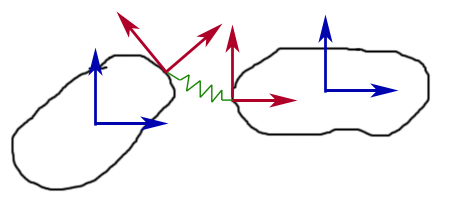
\includegraphics[width=0.30\textwidth]{softArt_G3.png}
	\caption{two bones linked by a joint-spring}
\end{figure}



\subsection{Sofa implementation}

To simulate these components in Sofa, we first need 2 mechanical objects : one for the bones (independent DOFs), and an other for the articulation points (mapped DOFs).
Each of them contains a list of rigid DOFs (respectively all the bones and all the articulations of the articulated body).
A mapping performs the link between the two lists, to know which articulations belong to which bones.


\subsubsection{Corresponding scene graph}
\begin{figure}[htpb]
	\centering
		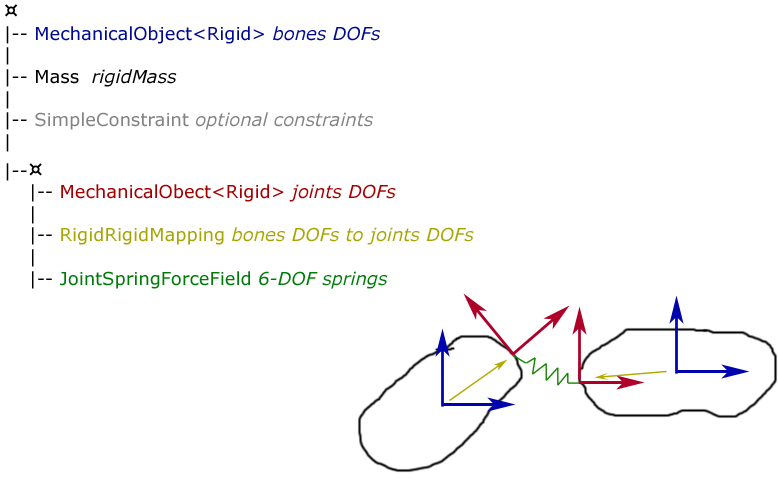
\includegraphics[width=0.90\textwidth]{scene_graph.png}
	\caption{a simple articulated body scene}
\end{figure}

\subsubsection {Example}

The example softArticulations.scn shows a basic pendulum :

\begin{verbatim}
<Node>
  <Object type="BruteForceDetection"/>
  <Object type="DefaultContactManager"/>
  <Object type="DefaultPipeline"/>
  <Object type="ProximityIntersection"/>

  <Node>
    <Object type="CGImplicitSolver"	/>
    <Object type="MechanicalObject" template="Rigid" name="bones DOFs"
            position="0 0 0  0 0 0 1 
                      1 0 0  0 0 0 1 
                      3 0 0  0 0 0 1 
                      5 0 0  0 0 0 1 
                      7 0 0  0 0 0 1" />
    <Object type="UniformMass" template="Rigid" name="bones mass"
            mass="1 1 [1 0 0,0 1 0,0 0 1]" />
    <Object type="FixedConstraint" template="Rigid" name="fixOrigin"
            indices="0" />
		
    <Node>
      <Object type="MechanicalObject" template="Rigid" name="articulation points"
              position="0 0 0  0.707914 0 0 0.707914 
                       -1 0 0  0.707914 0 0 0.707914 
                        1 0 0  0.707914 0 0 0.707914 
                       -1 0 0  0.707914 0 0 0.707914 
                        1 0 0  0.707914 0 0 0.707914 
                       -1 0 0  0.707914 0 0 0.707914 
                        1 0 0  0.707914 0 0 0.707914 
                       -1 0 0  0.707914 0 0 0.707914 
                        1 0 0  0.707914 0 0 0.707914" />
      <Object type="RigidRigidMapping"
              repartition="1 2 2 2 2" />
      <Object type="JointSpringForceField" template="Rigid" name="joint springs"
              spring="0 1   0 0 0 0 1 0   0 30000  0 200000   0  0 0 0  0 0 0 1 
                      2 3   0 0 0 0 1 0   0 30000  0 200000   0  0 0 0  0 0 0 1
                      4 5   0 0 0 0 1 0   0 30000  0 200000   0  0 0 0  0 0 0 1
                      6 7   0 0 0 0 1 0   0 30000  0 200000   0  0 0 0  0 0 0 1" />
    </Node>
    <Node>
      <Object type="MechanicalObject" template="Vec3d"
              position="-1 -0.5 -0.5  -1 0.5 -0.5 ..." />
      <Object type="MeshTopology"
              lines="0 1  1 2  ..."
              triangles="3 1 0  3 2 1  ..." />
      <Object type="TriangleModel"/>
      <Object type="LineModel"/>
      <Object type="RigidMapping"
              repartition="0 8 8 8 8" />
    </Node>
  </Node>
</Node>

\end{verbatim}

\begin{figure}[htpb]
	\centering
		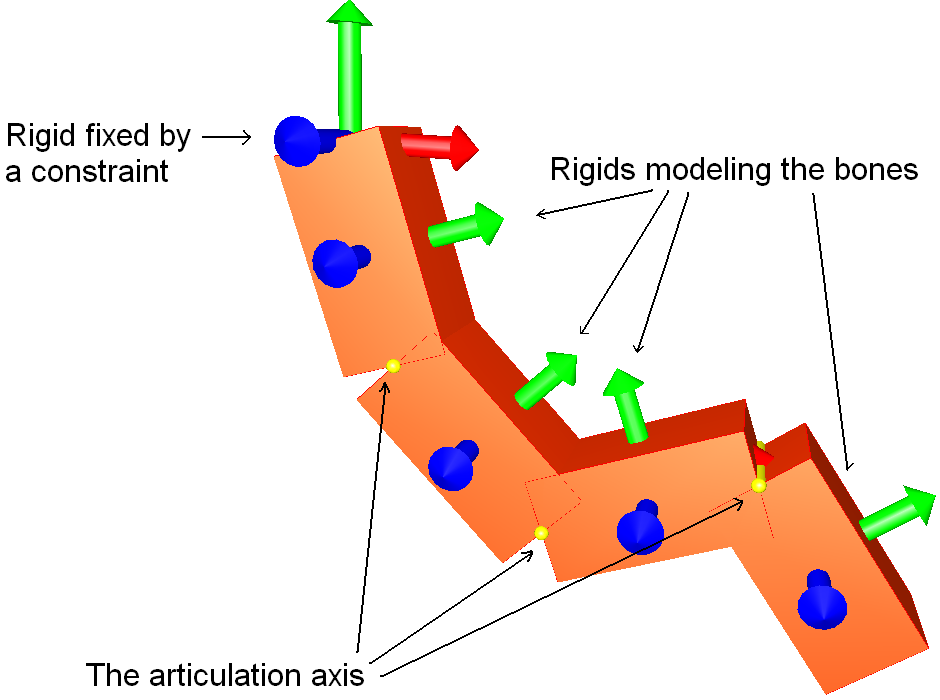
\includegraphics[width=0.70\textwidth]{softArt_snapshot.png}
	\caption{The pendulum is composed by 4 rigids linked one by one by articulations}
\end{figure}

In this example, we have under the first node the components to manage collisions, as usual.
Under the second node, we have :
\begin{itemize}
	\item the solver,
	\item the mechanical object modeling the independent rigid DOFs (5 rigids here),
	\item the rigid mass,
	\item a constraint, to fix the first rigid.
\end{itemize}

The third node (a child of the previous one) contains the components relative to the articulations :
\begin{itemize}
	\item the mechanical object modeling articulation points. Positions and orientations are relative to their parents.
	\item the mapping to link the two mechanical objects, as explained before. To know which articulations belong to which bones, a repartition vector is used. Several cases for this vector are possible :
		\begin{itemize}
			\item no value specified : every articulations belong to the first bone (classic rigid mapping).
			\item one value specified (ex: repartition="2") : each bone has the same number of articulations.
			\item number of bones values (like here, repartition="1 2 2 2 2") : the number of articulations is specified for each bone. For instance, here the first bone has 1 articulation, the next has 2 articulations, the next 2, Etc.
		\end{itemize}
	\item the JointSpringForceField containing the springs (4 springs here). Each spring is defined by a list of parameters. For instance for the first spring we have "0 1   0 0 0 0 1 0   0 30000  0 200000   0  0 0 0  0 0 0 1".
		\begin{itemize}
			\item "0 1" are the indices of the two articulations the spring is attached to
			\item "0 0 0 0 1 0" design the free axis for the movements. "0 0 0" mean that the 3 translation axis are constrained, and "0 1 0" mean that only the Y rotation axis is free.
			\item "0 30000 0 2000000" are the stiffnesses for each kind of movement: "0 30000" are respectively for free translation and for constrained translation", and "0 2000000" are respectively for free rotation and for constrained rotation.
			\item "0" is the damping factor
			\item "0 0 0" is to specify the initial translation
			\item "0 0 0 1" is to specify the initial rotation (quaternion)
		\end{itemize}
\end{itemize}

The last node contains the collision model. Nothing special here.


\subsection{Skinning}

The articulated body described previously models the skeleton of an object.
To have the external model (for the visual model or the collision model), which follows correctly the skeleton movements, it has to be mapped with the skeleton. 
\ 
A skinning mapping allows us to do this link. The external model is from this moment able to deform itself smoothly, i.e. without breaking points around the articulations.

The influence of the bones on each point of the external model is given by skinning weights.
2 ways are possible to set the skinning weights to the mapping :
\begin{itemize}
	\item Either the user gives directly the weights list to the mapping. It is useful if good weights have been pre computed previsouly, like in Maya for instance.
	\item Else, the user defines a number of references \textsl{n} that will be used for mapped points. Then, each external model point will search its \textsl{n} nearest bones (mechanical DOFs), and then compute the skinning weights from the relation :
\[ W = \frac{1}{d^{2}}  \]
\small{ with \textsl{d} : the distance between the external point and the rigid DOF.}
\end{itemize}

\begin{figure*}[htpb]
		\centering
		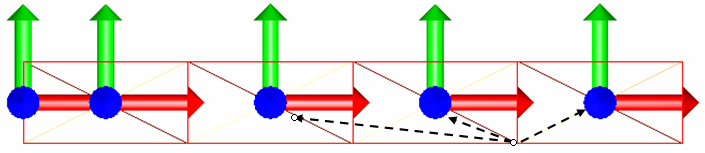
\includegraphics[width=0.50\textwidth]{skinning}
		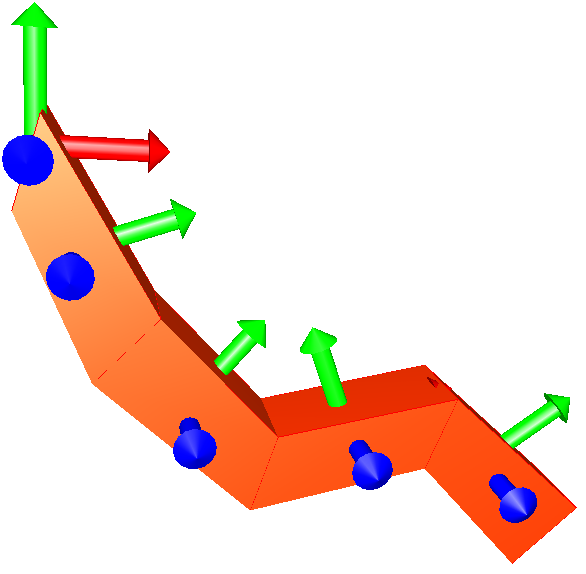
\includegraphics[width=0.30\textwidth]{skinnedPendulum}	
	\caption{In the example "softArticulationsSkinned.scn" the external points compute their skinning weights from the 3 nearest DOFs}
\end{figure*}

\section{Topology and Geometry}

% \subsection{Mesh topology}
While mesh geometry describes the location of mesh vertices in space, mesh topology indicates 
how vertices are connected to each other by edges, triangles or any type of mesh element. 
Both information are required on a computational mesh to perform mesh visualization,
mechanical modeling, collision detection, haptic rendering, scalar
or vectorial field description.

%Since topological changes are essential for surgery simulators, a common difficulty when designing those simulators is to ensure that the visual, mechanical, haptic and collision behavior of all meshes stay valid and consistent upon any topological change. 

% We handle topological changes in a modular and versatile way. Modular since each SOFA component (collision detection, mechanical solver$\ldots$) may be written with little knowledge about the nature of other components; versatile because any type of topological changes can be handled with the proposed design. 

Keeping a modular design implies that mesh related information (such as mechanical or visual properties) is not centralized in a single  mesh data structure but is instead spread out in the software components that are using this information.
% \\
% \textbf{\textit{Family of topologies}}\\
We consider meshes that are cellular complexes made of $k$-simplices (triangulations, tetrahedralisation) or $k$-cubes (quad or hexahedron meshes). These meshes are the most commonly used in real-time surgery simulation and can be hierarchically decomposed into $k$-cells, edges being $1$-cells, triangles and quads being $2$-cells, tetrahedron and hexahedron being $3$-cells. 
To take advantage of this feature, the  different mesh topologies are structured as a family tree (see Fig.~\ref{fig:BW_Topology_Family_Tree}) where children topologies are made of their parent topology. This hierarchy makes the design of simulation components very versatile since a component working on a given mesh topology type will also work on its derived types. For instance a spring-mass mechanical component only requires the knowledge of a list of edges (an \textit{EdgeSetTopology} as described in Fig.~\ref{fig:BW_Topology_Family_Tree}) to be effective. With this design, a spring-mass  component can be used at no additional cost on triangulation or hexahedral meshes that derive from an \textit{EdgeSetTopology} mesh.
 
%The proposed hierarchy makes also a distinction between conformal and manifold meshes. While most common FEM components require a mesh to be conformal (but not necessarily manifold), many high-level software components (such as cutting, contact, haptic feedback algorithms) require the mesh to be a manifold where a surface normal is well-defined at each vertex.   
\begin{figure}[ht]
    \centering
        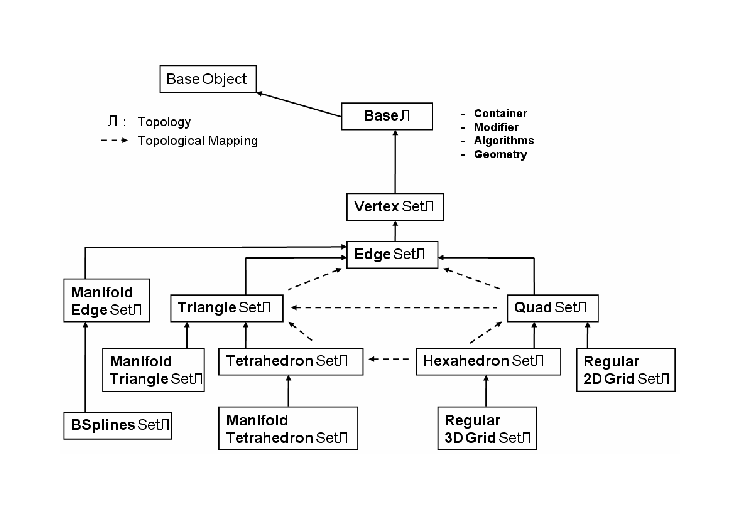
\includegraphics[width=0.9\textwidth]{BW_Topology_Family_Tree}
       \caption{Hierarchy of mesh topology. Dashed arrows indicate possible  \textit{Topological Mappings} from a topology object to another.}
    \label{fig:BW_Topology_Family_Tree}
\end{figure}


Topology objects are composed of four functional members:
 \textit{Container},  \textit{Modifier},  \textit{Algorithms} and  \textit{Geometry}.
The  \textit{Container} member creates and updates when needed two complementary arrays. The former describes the $l$-cells included in a single $k$-cell, $l<k$, while the latter gives the $k$-cells adjacent to a single $l$-cell.
From these arrays, generic methods give access to both full topological element description and complete adjacency information.
The  \textit{Modifier} member provides low-level methods that implement
elementary topological changes such as the removal or addition of an element. The  \textit{Algorithms} member provides high-level topological modification methods (cutting, refinement) which
decompose complex tasks into low-level
ones). 
The  \textit{Geometry} member provides geometrical information about the mesh (e.g. length, normal, curvature, ...) and requires the knowledge of the vertex positions stored in the  \textit{Degrees of Freedom} component. \\
%Note that these high-level changes may need geometrical information, such as mesh refining, triangular surface cutting or tetrahedra removal in a given region of interest.

\begin{figure}[ht]
    \centering
        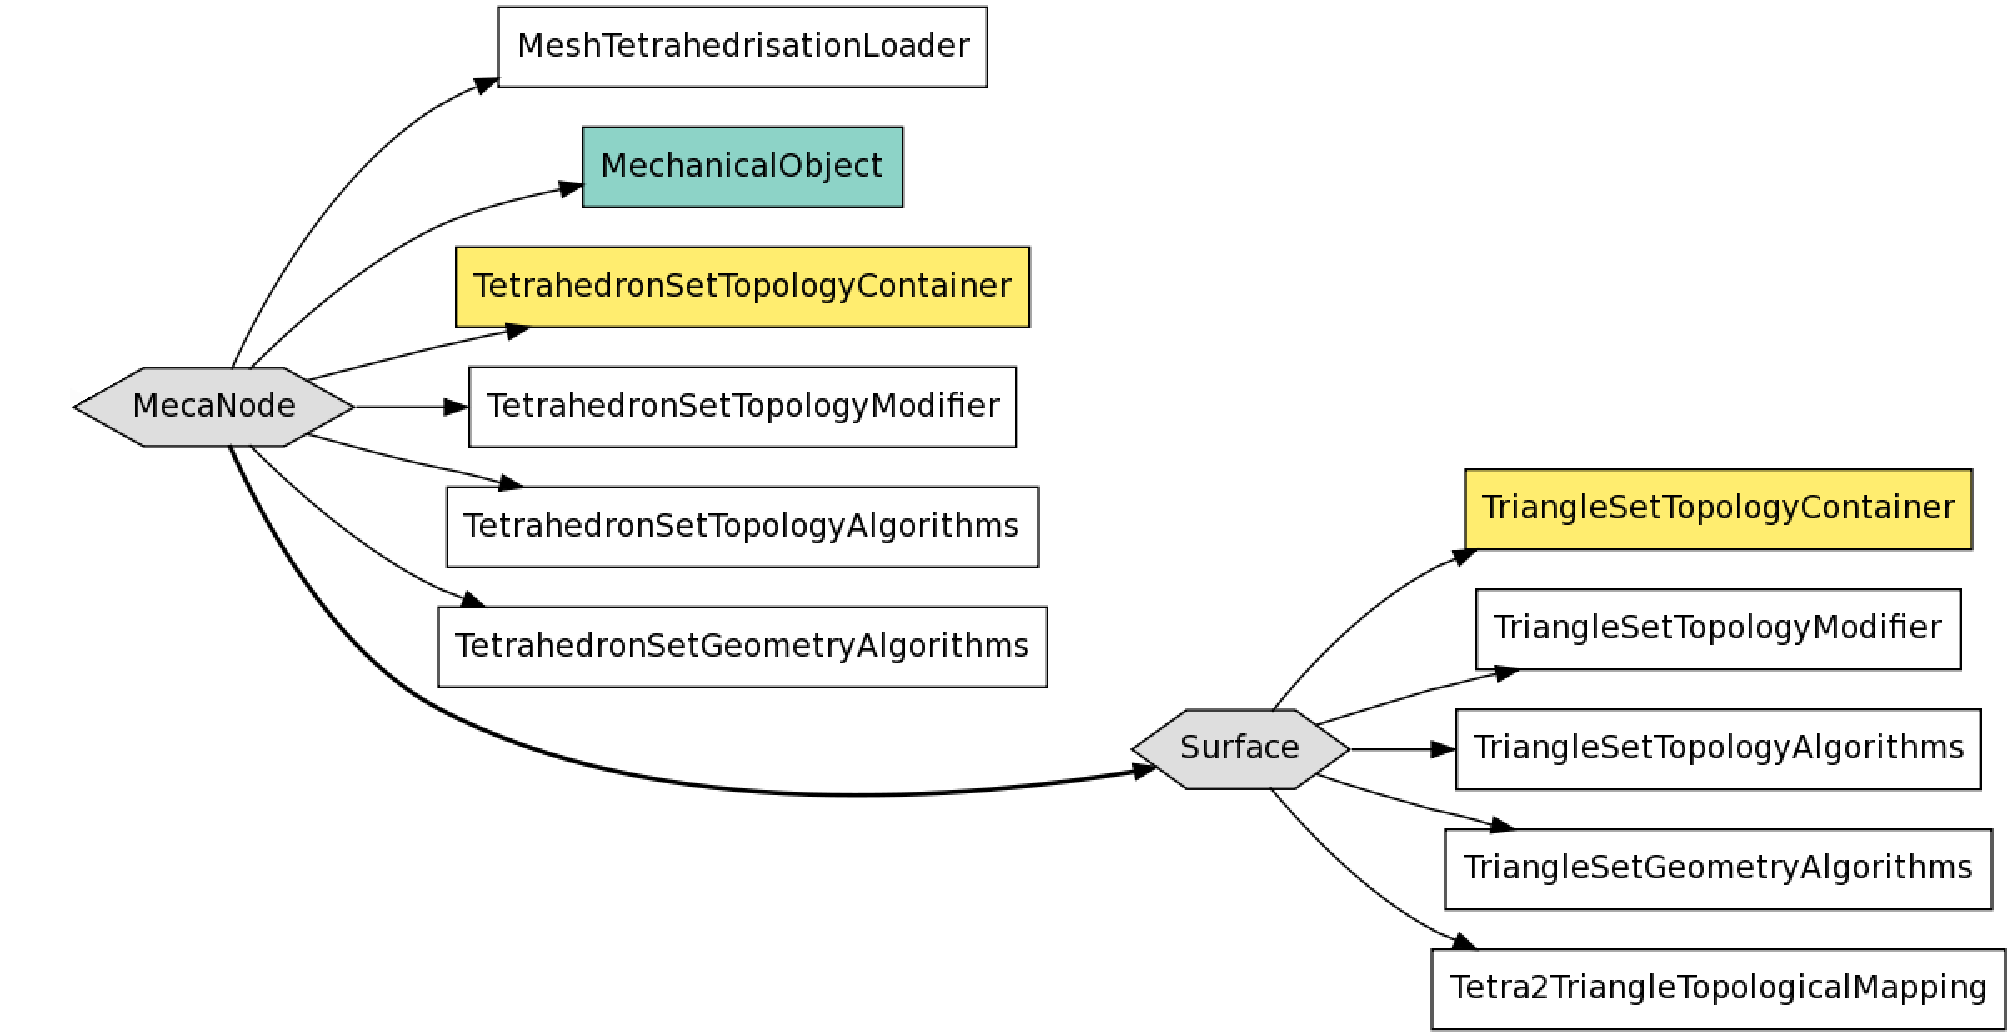
\includegraphics[width=0.9\textwidth]{topologyGraph.pdf}
       \caption{Scene Graph of a simple tetrahedral mesh where a topological mapping is defined to have the set of triangles located at the surface of the volumetric mesh.}
    \label{graphExample}
\end{figure}


Another important concept introduced in SOFA is the notion of \textit{Topological Mapping}. Those mappings  define a mesh topology in a from another mesh topology using the same DOFs.  For instance, one may need to apply specific forces on the surface bounding a volume (for instance to model the Glisson capsule surrounding the liver parenchyma). In this context, a \textit{Tetra2TriangleTopologicalMapping} may be used  to generate in a subnode the list of triangles on the border of a tetrahedral surfaces (see Figure \ref{graphExample}). Similarly, one may obtain the set of edges bordering a triangular mesh or the set of quads at the surface of an hexahedral mesh. Topological mapping may be used to split topological cells into other types of cells. Thus, a quad may be split into 2 triangles and an hexahedron into 5 or 6 tetrahedra. Specific mapping components exist to create an tetrahedral mesh from a set of hexahedra or to create triangular meshes from quads.

%An example of graph with Tetrahedral and Triangular Topology objects is given Fig. \ref{graphExample}. It also contains a mapping from the tetrahedral topology to the triangular one. 


\begin{figure}[ht]
    \centering
        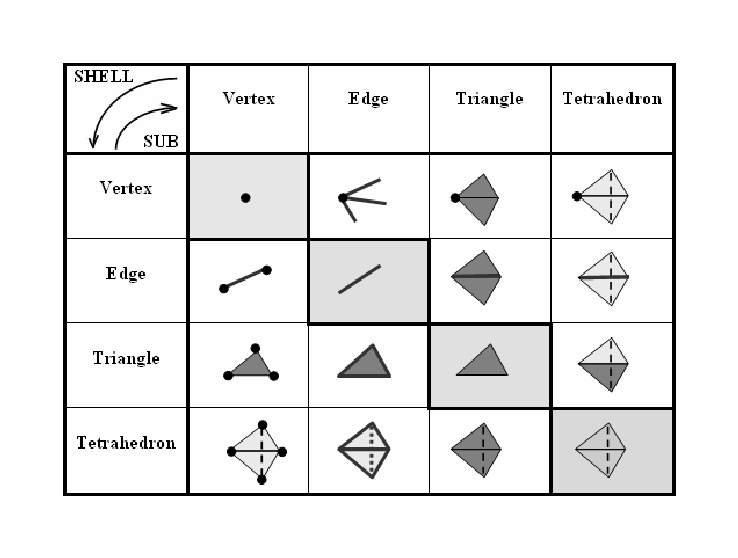
\includegraphics[width=0.8\textwidth]{BW_Sub_Shell_Diagram}
  %  \caption{Diagram of topological information for the elements of type Vertex, Edge, Triangle and Tetrahedron. \textit{ Sub Elements} (\textit{ bottom-left}) and \textit{ Shell Elements} (\textit{ top-right}) are stored in the \textit{ Container}. At each index $i$: \textit{ AB-Sub} array stores the indices vector of the elements of type \textit{ B} that compose the element of type \textit{ A} indexed by $i$; \textit{ AB-Shell} array stores the indices vector of the elements of type \textit{ A} that are adjacent to the element of type \textit{ B} indexed by $i$.}
    \caption{The two topological arrays stored in a \textit{ Container} correspond to the upper and lower triangular entries of this table. The upper entries provide the $k$-cells adjacent to a $l$-cell, $l<k$. The lower entries describe the $l$-cells included in a $k$-cell. Similar table exists for quad and hexahedron elements.}
    \label{fig:BW_Sub_Shell_Diagram}
\end{figure}

\subsubsection*{Mesh Data Structure}


% Choices of implementation
Containers storing mesh information (material stiffness, list of fixed vertices, nodal masses, ...) are stored in \textit{ components} and are spread out in the simulation tree.  
Most containers are simple arrays  with contiguous memory storage and a short direct access time.
This is important for real-time simulation, but bears some drawbacks when elements of these arrays are being removed since it entails the renumbering of elements. 
%For instance, when a single element is removed, the last array element is renumbered such that the array stays contiguous. 
Fortunately, all renumbering tasks that maintain consistent arrays can be automated and hidden to the user when topological changes in the mesh arise. 
Therefore, efficient access of  mesh data structures is granted while the complexity of keeping the container consistent with topological changes is automated.

There are as many containers as topological elements, currently: vertices, edges, triangles, quads, tetras, hexas. These containers are similar to the STL \textit{ std::vector} classes and allow one to store any component-related data structure. A typical implementation of spring-mass models would use an edge container that stores for each edge, the spring stiffness and damping value, the $i^{th}$ element of that container being implicitly associated with the $i^{th}$ edge of the topology. Finally, two other types of containers with similar characteristics have been defined. The former stores a data structure for a subset of topological elements (for instance pressure on surface triangles in a tetrahedralisation) while the latter stores only a subset of element indices.\\


%\subsubsection{Handling Topological Changes}\label{sec:topologicalChanges}

% to reformulate

% So as to make this design compatible with topological changes at each time step of the simulator,
% consistency has to be maintained for all components that rely on topology information, by applying the observer design pattern to the data structure.

% \subsection{Concept of Topological Event}

% \noindent % Order to respect when adding or removing an element (low-level methods)
% Motivation : topological changes are handled in a transparent way for the user through a mechanism of propagation of topological events from the topological components %toward other components.
%Surgery simulation involves complex topological changes on meshes, 
%for example when cutting a surface along a line segment, or when locally refining a volume before removing some tissue.
%However, one can always decompose these complex changes into a sequence of elementary operations, 
%such as adding an element, removing an element, renumbering a list of elements or modifying a vertex position.
%
%The approach used in \sofa to handle topological changes makes the  update of data structures transparent to the user, through a mechanism of propagation of topological events.
%A topological event corresponds to the intent to add or to
%remove a list of topological elements. But the removal of elements cannot be tackled in the same way as the addition of elements. Indeed, the element removal event must be first notified to
%the other components before the element is actually removed by the \textit{Modifier}.
%Conversely, element addition is first processed by the \textit{Modifier} and then element addition event is notified to other components.
%Besides, the events notifying the creation of elements also include a list of ancestor elements. Therefore, when splitting one triangle into two sub-triangles, each component-related information (\textit{ e.g.} its Young modulus or its mass density) associated with a sub-triangle will be created knowing that the sub-triangle originates from a specific triangle. Such mechanism is important to deal with meshes with non-homogeneous characteristics related to the presence of pathologies.
%
%\vspace{-0.5cm}
%
%\begin{figure}[ht]
%    \centering
%      %  \mbox{
%      %  \includegraphics[width=0.5\textwidth]{Handling_Topological_Changes}
%      %    \includegraphics[width=0.5\textwidth]{Triangle_Splitting}
%      %  }
%        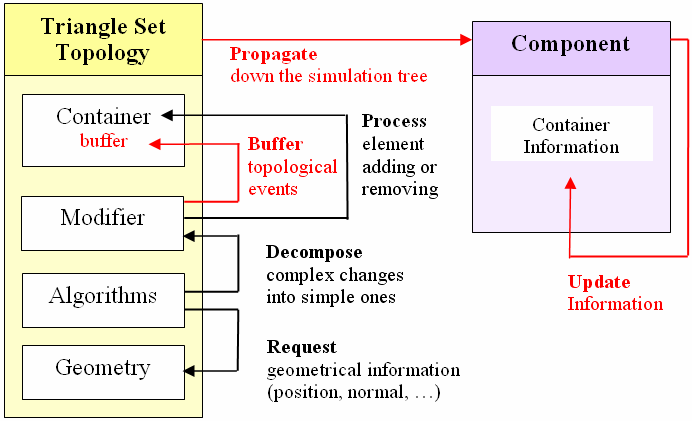
\includegraphics[width=0.8\textwidth]{Handling_Changes}
%    \caption{Handling topological changes, with the example of a \textit{Triangle Set Topology}. 
%   \textit{Component} corresponds to any component of the simulation which may need topological information to perform a specific task.
%    Black features indicate the effective change process. Red features show the steps of event notification.}
%    \label{fig:Handling_Changes}
%\end{figure}


% \vspace{-1.5cm}

%\begin{figure}[ht]
%    \centering
      %  \mbox{
      %  \includegraphics[width=0.5\textwidth]{Handling_Topological_Changes}
      %    \includegraphics[width=0.5\textwidth]{Triangle_Splitting}
      %  }
%        \includegraphics[width=0.65\textwidth]{Triangle_Splitting}
%    \caption{Seven steps to split one triangle into two sub-triangles.}
%    \label{fig:Triangle_Splitting}
%\end{figure}

%The mechanism to handle topological changes is illustrated by Fig.~\ref{fig:Handling_Changes}.
%The notification step consists in accumulating the sequence of
%topological events  involved in a high-level topological change into a buffer stored in
%the \textit{ Container}. Then the event list is propagated to all its
%neighbors and leaves beneath by using a visitor mechanism, called a
%\textit{ Topology Visitor}. Once a given component is visited, the topological
%events are actually processed one by one and the data structure used to store mesh related information are automatically updated.
%
%In practice, for each specific component (\textit{ e.g.} spring-mass mechanical component), a set of callback functions are provided describing how to update the data structure (\textit{ e.g.} spring stiffness and damping values) when adding or removing an element (\textit{ e.g.} the edges defined by the two extremities of the springs).
%We applied the observer design pattern so that component-related data structures update themselves automatically.




\newpage
\section{Graphic User Interface}
\subsection{First steps}
\par
Once SOFA is compiled, in the directory bin will be placed an executable called runSofa (or runSofad if you are using the debug version).
The first time you will run SOFA, a GUI using Qt will appear. By default a simulation modeling a liver with some fixed points will be displayed. Simulations must be written in a xml format, generally, Sofa scenes have the extension ``.scn'', and Sofa objects directly the extension ``.xml''. You can load both of them using the file menu, or drag \& dropping them in the interface.\\
Basically the GUI is divided in two: 
\begin{itemize}
 \item a control panel subdivided in several tabulations, giving the user the possibility to display various information about the simulation, and even modifying it interactively
 \item a viewer: by default, you will be using our hand-made viewer, using OpenGL. Others are available, and below, we describe how to create your own viewer, if you desire to insert a more powerful rendering engine.
\end{itemize}

\begin{figure}[htpb]
	\centering
		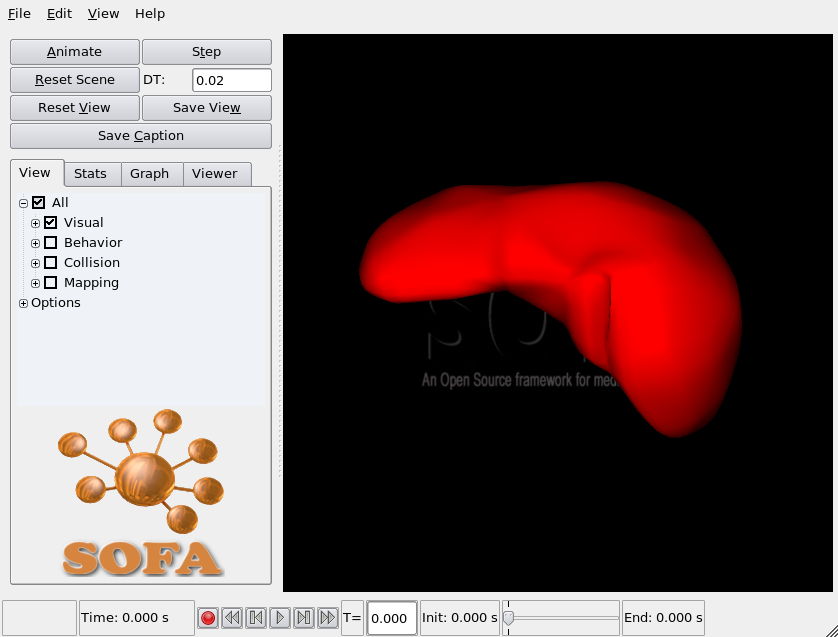
\includegraphics[width=1.0\textwidth]{GUI/GUI.png}
	\caption{SOFA first-time}
\end{figure}
At any time, you can hide the control panel by moving its right border to the left.
\newline

\par

\begin{figure}
	\centering
		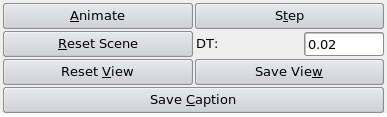
\includegraphics[width=0.45\textwidth]{GUI/GUI_basic.png}
	\caption{Basic Controls}
\end{figure}\begin{center}

\vspace{25mm}            \end{center}
The basics controls are :
\begin{itemize}
 \item {\bf Animate} : launch the simulation. The simulation won't stop until you press Animate.
 \item {\bf Step}: Process only one step of the simulation. 
 \item {\bf Reset Scene}: Reset all the components to their initial values.
 \item {\bf Reset View}: Reset the camera to its original place.
 \item {\bf Save View}: Save the position and orientation of the camera. Next time you will load your scene, these information will be used.
 \item {\bf Save Caption}: Take a screenshot of the current simulation.
\end{itemize}

DT corresponds to the time step used in the computation of the simulation. It can be changed interactively.










\subsection{View Tab}
The ``View Tab'' is the default tab, you can filter the information you want to be displayed by your viewer. It is quite useful to have a fast and global control. 

\begin{figure}[htpb]
	\centering
		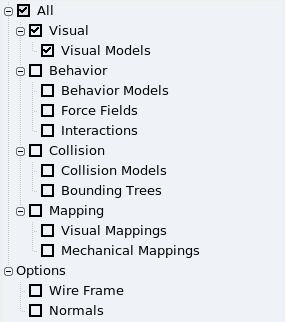
\includegraphics[width=0.3\textwidth]{GUI/GUI_visual.png}
	\caption{Basic Controls}
\end{figure}

The options are:
\begin{itemize}
 \item {\bf All}: Enable or disable the display of all the visual information available in SOFA
 \item {\bf Visual Models}: the graphic representation of the objects
\item {\bf Behavior Models}: the mechanical DOFs of the simulation
\item {\bf Collision Models}: the models used to perform the collision detection
\item {\bf Bounding Tree}: the hierarchical bounding boxes of the collision models
\item {\bf Mappings}: All the non-mechanical mappings (for instance the visual mappings that link a mechanical object to its visual representation)
\item {\bf Mechanical Mappings}: All the mechanical mapping that propagates the forces and position from a mechanical object to another
\item {\bf Interactions}: Interactions of all kind between objects. Some are created by the collision pipeline when a penalty response is used
\item {\bf Wire Frame}: Change the way 3D models(visual, and collision) are displayed
\item {\bf Normals}: Normals of the visual models
\end{itemize}








\subsection{Stats Tab}
The ``Stats Tab'' is a tab displaying an inventory of the collision models present in the scene( how many triangles, lines, points, spheres, are used to perform the collision detection). You can also output some information about the current simulation. 
\begin{itemize}
 \item Dump State: export in ``dumpState.data'' the state of the simulation
 \item Log Time: display in the console, the time spent in each step of the simulation. Useful to do some monitoring
 \item Gnuplot: export gnuplot files. It will export positions, velocities, energies. Files will have the same name as the Object associated in the simulation, following by:
\begin{itemize}
 \item {\bf ``\_x''} for the positions
 \item {\bf ``\_v''} for the velocities
 \item {\bf ``\_Energy''} for the Energies (contains kinetic, potential and mechanical)
\end{itemize}

You can specify the directory where you want the files to be saved in the menu Edit.
\end{itemize}











\subsection{Graph Tab}
The ``Graph tab'' is certainly the most important tab. It displays the scene graph of the simulation. You can quickly see all the components used in the current simulation. The ``Export Graph...'' button gives a graphic representation of the inter-dependencies of the objects.

\begin{figure}[htpb]
	\centering
		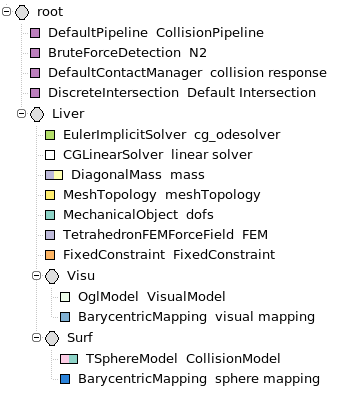
\includegraphics[width=0.5\textwidth]{GUI/GUI_graph.png}
	\caption{Scene Graph for the liver scene}
\end{figure}

This graph can dynamically change during the simulation: collisions can create new nodes, new components in case of contacts. But you can directly interact with it too. Double clicking on an item of the graph will make appear a small window displaying important data.

To know how to display the information of your brand new Sofa component, please refer to the section ``How to configure your Component''. Only objects of type ``sofa::core::objectmodel::Data'' or ``sofa::core::objectmodel::DataPtr'' can be displayed. It is important to understand that only these information will be kept if you decide to save the simulation. Loading a saved simulation, will just fill the components with this data.
This kind of dialog windows give the possibility to modify directly some characteristics of your component. Take care to click on the button ``Update'' once you have completed your modifications.

\begin{figure}[htpb]
	\centering
		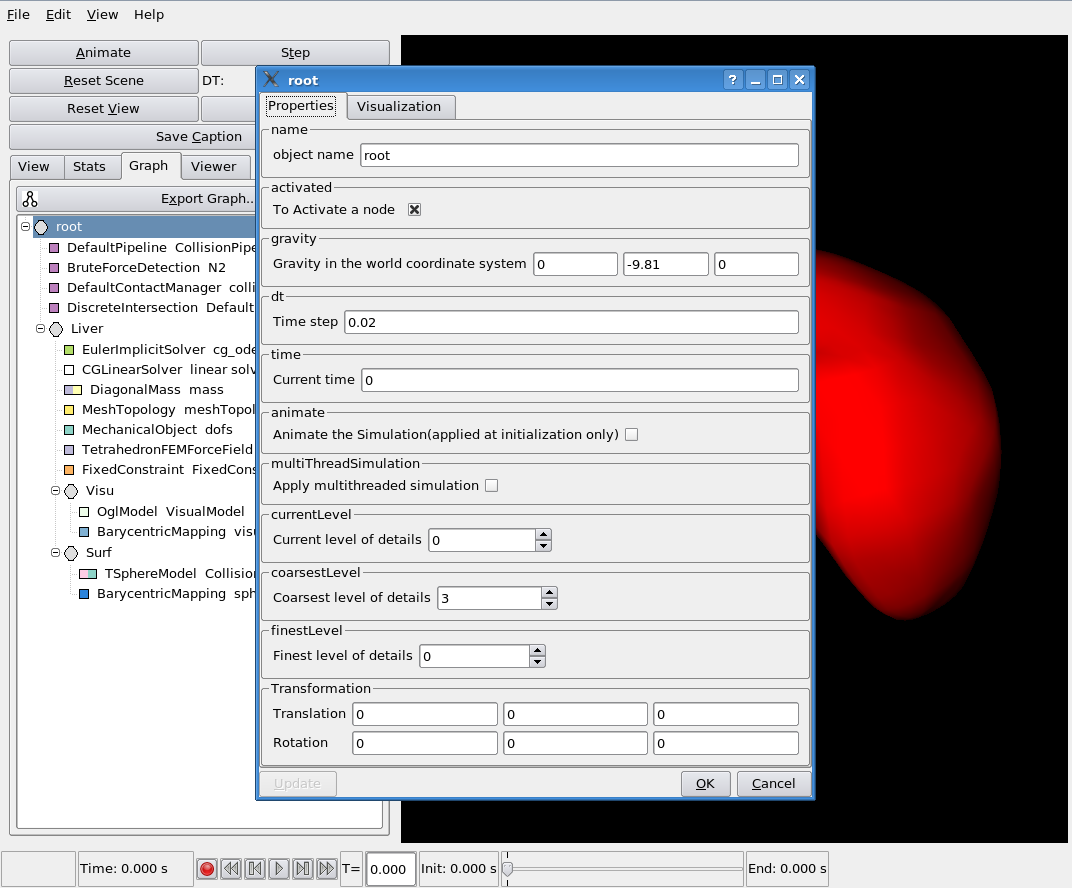
\includegraphics[width=0.8\textwidth]{GUI/GUI_modify.png}
	\caption{Double click on an item of the graph}
\end{figure}

\par
A Node gives access to much more interactions: right clicking on one of them makes appear a small context window.
\begin{itemize}
 \item {\bf Collapse}: Collapse the graph from the current node, close all the nodes below the clicked one
 \item {\bf Expand}: Expand the graph, and open all the nodes below the clicked one
 \item {\bf Desactivate}: Deactivate a part of the scene. Everything below this node won't be anymore taken into account. BUT it remains in the scene, and can be Activated again at any time
 \item {\bf Save Node}: Export in a XML files a part of the simulation
 \item {\bf Add Node}: Read a XML files describing an object or a whole scene, and put it right below the clicked node.
An interesting feature to note, is when you might be always using, and adding the same set of objects, you will find it convenient to add in the file scenes/object.txt the path to them. Like this, they will directly appear in the dialog window by default.
 \item {\bf Remove Node}: Remove from the simulation everything within the clicked node. You won't be able anymore to make it appear unless you proceed to a restart or reload of the scene.
 \item {\bf Modify}: Open the same dialog window as might do a double click: this action is common to all the items of the graph
\end{itemize}

\begin{figure}[htpb]
	\centering
		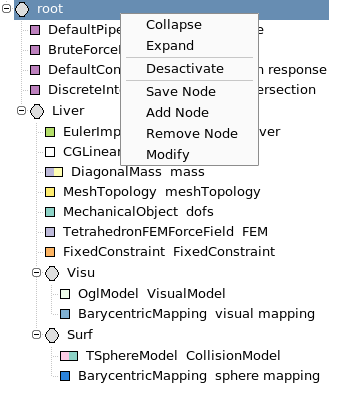
\includegraphics[width=0.4\textwidth]{GUI/GUI_interaction.png}
	\caption{Right click on a node of the graph}
\end{figure}








\subsection{Viewer Tab}
The ``Viewer tab'' describes all the keyboard shortcuts available for the current viewer.

The last useful option of this tab is the possibility to re-size your viewer, which can be very helpful to record a video at a given resolution.









\subsection{Interactions}
You can interact with the simulation using the mouse with SHIFT + Right Click. A ray will be cast, and if it intersects one collision model of the scene, a spring will be created, allowing you to pull on some elements of the scene.



\newpage
\subsection{Architecture}
Fig.~\ref{fig:GUI_UML} gives an overview of the modular architecture of the GUI for SOFA. 
\begin{figure}[htpb]
	\centering
		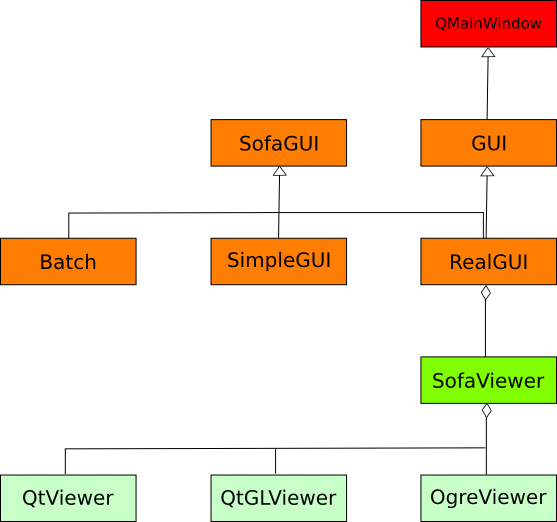
\includegraphics[width=0.9\textwidth]{GUI/GUI_UML.png}
	\caption{A modular Architecture of the GUI}
 	\label{fig:GUI_UML}
\end{figure}








\subsection{Change the viewer}
By default, SOFA provides three viewers, that can be integrated easily to the Qt interface. 

\begin{itemize}
 \item {\bf QtViewer}: a hand made viewer using OpenGL functionality
 \item {\bf QtGLViewer}: a viewer using the library QGLViewer created by Gilles Debunne. It is distributed directly with SOFA, but you can also download it at:\\ {\bf http://artis.imag.fr/Members/Gilles.Debunne/QGLViewer/}
 \item {\bf OgreViewer}: this viewer remains experimental, but shows how it is possible to integrate a powerful rendering engine such as OGRE3D. You need to install Ogre. You can download it at {\bf http://www.ogre3d.org}.
\end{itemize}

To use them, you have to edit the file sofa-default.cfg located in your SOFA directory, and uncomment the lines corresponding to the viewer you want. If you have several viewers activated, you can launch SOFA with a specific one by using the option:
\begin{itemize}
 \item ``runSofa -g qt'' : for QtViewer
 \item ``runSofa -g qglviewer'' : for QtGLViewer
 \item ``runSofa -g ogre'' : for OgreViewer
\end{itemize}

You can also dynamically change the viewer when SOFA is running. The menu View of the main window displays all the viewer available and let you switch at any time.
\par
If you desire to create a new viewer, the first step is to make it derive from SofaViewer. 








\subsection{Choose the GUI}
By default, Sofa provides three GUIs.
\begin{itemize}
 \item {\bf Batch}: no gui, proceeds to 1000 iterations and then stops
 \item {\bf GLUT}: GLUT window, implementing only the basic functions. To start the animation, you have to pass the option ``-s'' to your runSofa
 \item {\bf Qt}: the default GUI, already described above
\end{itemize}

The Batch GUI is always available. To use GLUT or Qt interface, you have to uncomment in sofa-default.cfg the corresponding lines. To use them
\begin{itemize}
 \item ``runSofa -g batch'' : for no GUI
 \item ``runSofa -g glut'' : for GLUT window 
 \item for Qt GUI, please refer to the section above. By default, Sofa is using Qt interface with QtViewer.
\end{itemize}
If you desire to create a new GUI, the first step is to make it derive from SofaGUI. 






\subsection{Player/Recorder}

\begin{figure}[htpb]
	\centering
		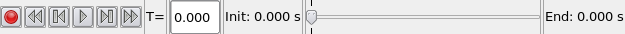
\includegraphics[width=0.7\textwidth]{GUI/GUI_recorder.png}
	\caption{Player/Recorder in Sofa} 	
\end{figure}
Sofa provides with the Qt Graphic interface, a compact Player/Recorder of simulation. When you want to record a simulation, press the red button (record). Automatically, some components will be added to your graph, and will create files to save the position, and velocities of all your mechanical elements. To stop recording, press again on the record button. A file with the same name as your simulation will be created, but with the extension ``.simu''. Sofa is able to read these files, and will initialize correctly the Player. 
\par
To readback a recorded simulation, you can process to a step by step(forward, and backward), or a continuous play. You can jump to a specific moment of your recording. You can even change the Dt of the recording, if you want to accelerate, or reduce the velocity of the playing. At any time, you can animate the scene (by pressing the Animate button), to compute the simulation. 
\par
The files will be stored by default in the directory scenes/simulation of your SOFA. Nevertheless, you can change this directory by clicking on the menu Edit of the main window.







\section{Modeler}
A modeler for Sofa has been recently created. The purpose of this tool is both to help the new-comers in Sofa to get an overview of the whole framework, and accelerate the process of creation and configuration of a complex simulation for expert users.
\begin{figure}[htpb]
	\centering
		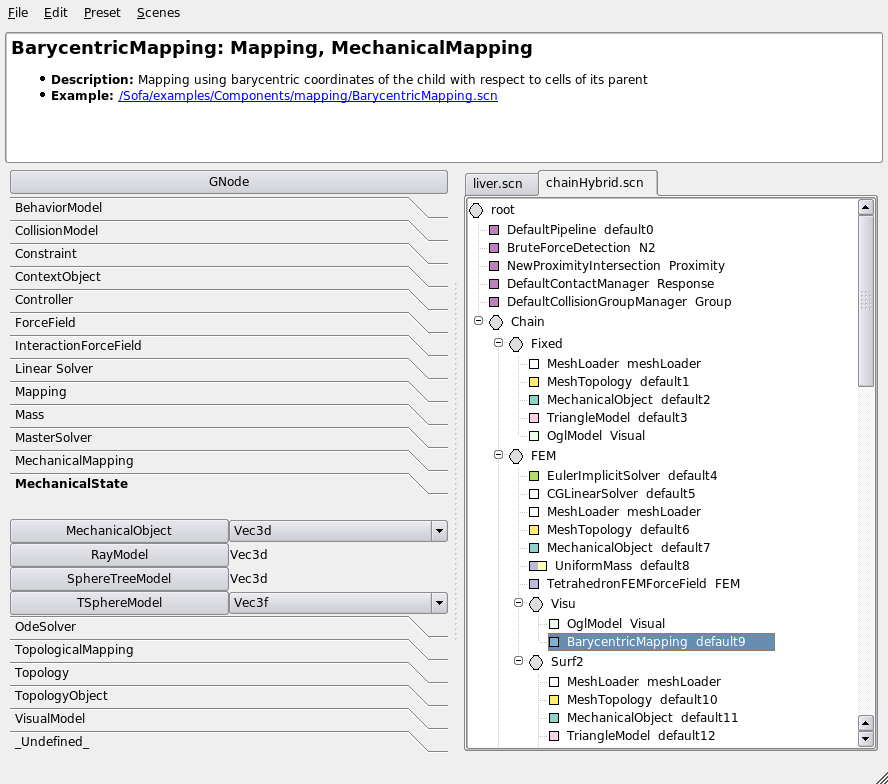
\includegraphics[width=0.75\textwidth]{GUI/Modeler.png}
	\caption{Main Window of the Modeler} 	
\end{figure}

\subsection{Library}
The left part of the application displays a library of all the different components available in Sofa, sorted by the name of the Base Class. Clicking on any of them will display information about the usage, authors, licence if any, and sometimes a link to an example. This link will open a new tab in the modeler displaying a simulation. 
At any time, you can launch Sofa from the Modeler, hitting CTRL+R, or going to File ... Run In Sofa.
\subsection{Graph Editor}
The right part seems very similar to the scene graph displayed in Sofa. The behavior is the same. Double clicking on a component will open a dialog, in which you can define all the parameters of the object. But, as you are in an editor, you can easily remove everything you have added. This editor is very convenient to test things. Try to create your object, launch into sofa, modify some components, or parameters, using the documentation displayed each time you select one item. 
\subsection{Modeling}
To model a new scene, just make a series of drag and drop of the components you desire from the Library to the Graph Editor. By default, when opening a new tab, all the default components to perform the collision detection are added. If you don't want them, just clear the tab (CTRL+N).\\
To accelerate the process of creation, preset objects are available. You can build automatically :
\begin{itemize}
  \item deformable objects
  \begin{itemize}
    \item in a grid
    \item using a tetrahedral mesh
  \end{itemize}
  \item rigid objects  
  \begin{itemize}
    \item simulated
    \item not simulated: they will perform as obstacle like floors, or walls
  \end{itemize}
\end{itemize}



\newpage

\section{Light management}

One white global light illuminates the scene by default. This can be changed
through a light manager object and a certain number of lights (limited by
OpenGL).

The first step is to add the object called ``LightManager'', preferably at the
top of the scene file.
\begin{code_xml}
	<Object type=``LightManager'' />
\end{code_xml}

After that, we can add 3 different kinds of lights :
\begin{itemize}
  \item a positional light (parameters : color, position) ;
	\begin{figure}[!h]
	\centering
	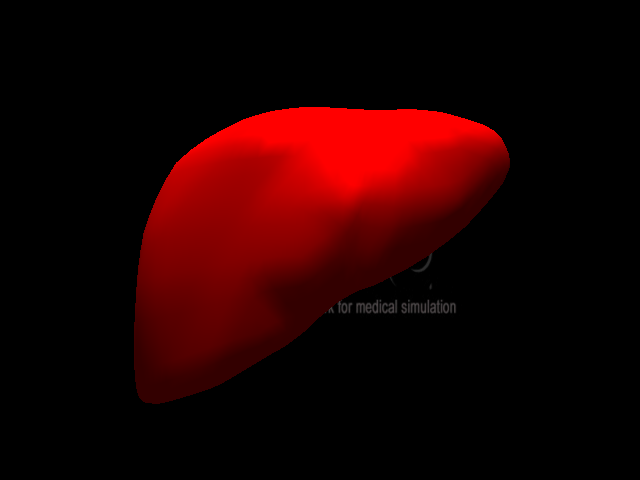
\includegraphics[width=0.33\linewidth]{rendering/images/light_pos.png}
	\caption{Positional Light}
	\end{figure}

	\begin{code_xml}
		<Object type="PositionalLight" position="0 -5 10" />
	\end{code_xml}
%\newpage
  \item a directional light (parameters : color, direction) ; 
	\begin{figure}[!h]
	\centering
	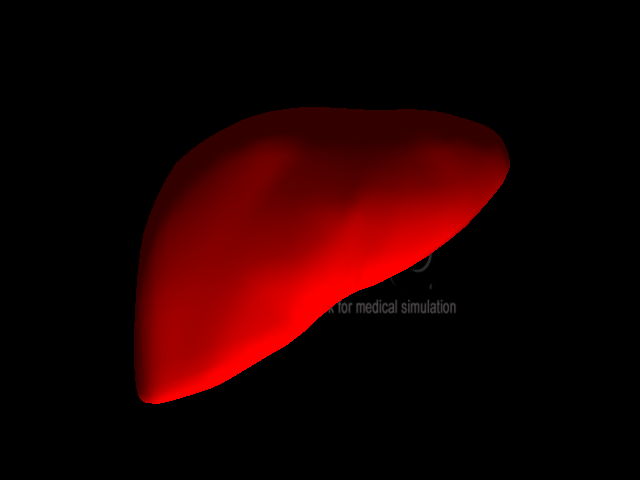
\includegraphics[width=0.33\linewidth]{rendering/images/light_dir.png}
	\caption{Directional Light}
	\end{figure}

	\begin{code_xml}
		<Object type="DirectionalLight" direction="0 5 0" />
	\end{code_xml}
\newpage

  \item and a spotlight (parameters : color, position, direction, cut off,
  exponent, attenuation)

	\begin{figure}[!h]
	\centering
	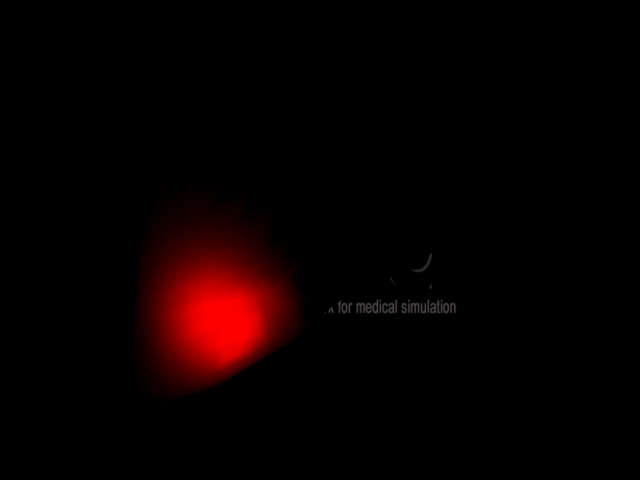
\includegraphics[width=0.33\linewidth]{rendering/images/light_spot.png}
	\caption{Spot Light}
	\end{figure}

	\begin{code_xml}
		<Object type="SpotLight" position="-3 2 5" direction="0 0 -1" />
	\end{code_xml}
\end{itemize}

\section{Shader management}
A complete set of tools about using shaders is implemented into SOFA. The three kinds of shaders (vertex and fragments (mandatory), geometry (optionally)) are available.
Shader is used only for Visual Model as OglModel.
\newline
The effects of the shader is spread to the associated subtree.
Finally, there is only one shader activated for each visual model : if two shaders are present in the same node, only the second will be effective.

	\begin{figure}[!h]
	\centering
	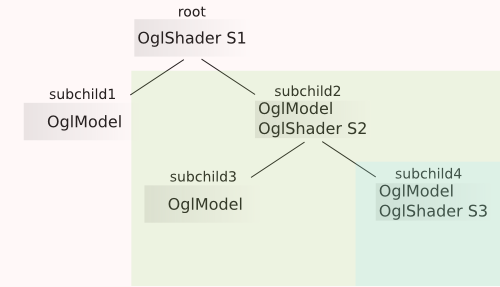
\includegraphics[width=0.8\linewidth]{rendering/images/shader_tree.png}
	\caption{Example of shaders' area of effect}
	\end{figure}

To simply include a shader, add this into your node :
	\begin{code_xml}
		<Object type="OglShader" vertFilename=``test.vert'' fragFilename=``test.frag'' />
	\end{code_xml}

\textit{vertFilename} and \textit{fragFilename} are the only mandatory parameters. Other optional parameters are about geometry shader : \textit{geoFilename}, \textit{geometryInputType}, \textit{geometryOutputType} and \textit{geometryVerticesOut}. A last parameter, \textit{turnOn}, is for debugging purpose, when you want to disable shader without restarting the scene.

If you want to send values to uniform variables defined into the shader, a certain number of objects is available : 
\begin{itemize}
 \item OglIntVariable,OglInt{2,3,4}Variable : for int and ivec{2,3,4}
 \item OglFloatVariable,OglFloat{2,3,4}Variable : for float and vec{2,3,4}
 \item OglIntVectorVariable, OglIntVector{2,3,4}Variable : for arrays of int and ivec{2,3,4}
 \item OglFloatVectorVariable, OglFloatVector{2,3,4}Variable : for arrays of float and vec{2,3,4}
\end{itemize}

Their parameters are \textit{id} for their name into the shader and \textit{value} (single type) or \textit{values} (array type).
Example : 
	\begin{code_xml}
		<Object type="OglFloat3Variable" id="fragmentColor" value="1.0 0.0 0.0" />
		<Object type="OglFloatVariable" id="fragmentOpacity" value="2.0"/>
		<Object type="OglFloatVector4Variable" id="MappingTable" values="1.0 0.0 0.0 0.0 0.0 0.0 0.0 1.0" />
	\end{code_xml}

2D texture can be added with OglTexture2D object.Its parameters are \textit{id}, \textit{texture2DFilename} and \textit {textureUnit}.

	\begin{code_xml} 
		<Object type="OglTexture2D" texture2DFilename="textures/lights4-small-noise.bmp" textureUnit="1" id="planeTexture" />
	\end{code_xml}

The last object about shaders is a partial support of macro processing in GLSL. It's possible to define macro variable if a part of code is enabled or not. For example, this can be very useful if there is a common code for two 3D objects, one with a texture, and the other with simple colors. You define the macro :

	\begin{code_cpp} 
		#define HAS_TEXTURE
			...;
			//code about textured 3D object
		#else
			...;
			//code about colored 3D object
		#endif
	\end{code_cpp}

and put the following object into the scene file, at the same node as the OglShader used by the textured 3D object:

	\begin{code_xml} 
		<Object type="OglShaderDefineMacro" id="HAS_TEXTURE" />
	\end{code_xml}






\end{document}          

